%%%%%%%%%%%%%%%%%%%%%%%%%%%%%%%%%%%%%%%%%%%%%%%%%%%%%%%%%%%%%%%%%%%%%%%
% Based on IEEE the conference template available                     %
% at https://www.ieee.org/conferences/publishing/templates.html       %
% Adapted for the Data Science Lab course at Politecnico di Torino    %
% by Giuseppe Attanasio, Flavio Giobergia                             %
% 2020, DataBase and Data Mining Group                                %
%%%%%%%%%%%%%%%%%%%%%%%%%%%%%%%%%%%%%%%%%%%%%%%%%%%%%%%%%%%%%%%%%%%%%%%

\documentclass[conference]{IEEEtran}
\usepackage{cite}
\usepackage{amsmath,amssymb,amsfonts}
\usepackage{algorithmic}
\usepackage{graphicx}
\usepackage{textcomp}
\usepackage{xcolor}
\usepackage{url}

\begin{document}

\title{Prediction of particle position passing through a sensor with multiple readings}

\author{\IEEEauthorblockN{Michele Moneta, Alex Vellone}
\IEEEauthorblockA{\textit{Politecnico di Torino} \\
Student id: s317492, s331792 \\
\{s317492, s331792\}@studenti.polito.it}
}

\maketitle

\begin{abstract}
This report presents a data science pipeline using scikit-learn Random Forest Regressor to 
predict particle positions based on multiple signals measured by a Resistive Silicon Detector.
\end{abstract}


\section{Problem overview}
In the particle physics field, the detection of the position of a particle is something physicists face continuously. 
This can be done with various types of sensors. In this specific case a \textit{RSD (Resistive Silicon Detector)} 
was used. This type of sensor has a 2-dimensional surface within which it can detect the passage of particles.
The RSD sensor has 12 “snowflake” shaped metallic pads that are used to measure \textit{signals}. 
When a particle traverses the sensor, signals are generated by these pads, forming the basis for predicting 
the particle's (x, y) coordinates.

For every signal measured by the pads we can extract some features:
\begin{itemize}
    \item pmax (positive peak magnitude): the magnitude of the positive peak of the signal, measured in millivolts (mV). 
    This represents the maximum amplitude of the positive part of the signal.
    \item negpmax (negative peak magnitude): the magnitude of the negative peak of the signal, measured in millivolts (mV). 
    This represents the maximum amplitude of the negative part of the signal.
    \item tmax (delay of positive peak): the delay, measured in nanoseconds (ns), from a reference time to when 
    the positive peak of the signal occurs. 
    This indicates the time at which the peak of the positive signal is reached.
    \item area (area under the signal): the area under the signal curve.
    This provides information about the total charge or energy deposited by the particle as it passes through the detector.
    \item rms (root mean square): the rms value of the signal.
\end{itemize}

Figure \ref{fig:sensor_reading} shows a representation of a signal measured by a pad with all the features 
that can be extracted from it.\\
\begin{figure}[htbp]
\centerline{\includegraphics[width=\linewidth]{media/sensor_signal.png}}
\caption{Signal measured by a pad of the sensor.}
\label{fig:sensor_reading}
\end{figure}

The sensor output contains 18 readings of the event. Since only 12 pads are available, some of the 
readings are noise and does not contain actual readings.

The dataset contains 514,000 events, each providing 18 readings from the 12 pads. 
For each event the passage of a particle has been enforced (i.e. the (x,y) coordinates are known) 
and are available in the dataset.

This multi-output regression problem involves predicting the (x, y) coordinates of particles as they 
pass through a Resistive Silicon Detector (RSD), using the provided (x, y) coordinates and the 
pads readings as the evaluation set. 
The task requires analyzing the dataset and developing a data science pipeline to forecast particle 
coordinates from sensor readings, utilizing insights gained from the training dataset.\\

The dataset is composed by two files:
\begin{itemize}
    \item development.csv: a comma-separated values file containing the 385,500 events for the development set.
    \item evaluation.csv: a comma-separated values file containing the 128,500 events 
    corresponding to the evaluation set. 
    This portion does not contain the (x,y) coordinates.
\end{itemize}

For the evaluation a third csv file need to be created, This file will contain 128,500 (x,y) 
predictions of the evaluation dataset.
This file will be uploaded for the final exam score.


\section{Proposed approach}
The initial phase of our approach involves an exploration of the dataset.
This exploratory analysis aims to unveil patterns within the sensor readings.
Following dataset exploration, an analysis is conducted to discern the importance of
each extracted feature of each pad.

To enhance the model's precision, pads that introduce noise need to be removed from the dataset. 
This ensures that the regression model is trained exclusively on usefull information, 
refining the dataset for optimal performance.


\subsection{Preprocessing}
A first look at the dataset reveals that it is composed of 92 columns. 
It contains 5 features for every of all the 18 pads.
Plus two columns for the x and the y coordinates.
A preliminary exploration into the x and y columns discloses values within the 200 to 600 range, 
all of which are multiples of 5. Consequently, the x and y columns contain 81 distinct values.

In figure \ref{fig:cartesian_plane}, each event of the evaluation dataset is collocated on a Cartesian plane 
using the x and y coordinates. Looking at the image it is possible to see that there are five distinct areas, 
or “holes”, where there is an absence of data.
This pattern evokes the sensor image described in the problem statement, suggesting that these 
“holes” might correspond to areas where the pads are incapable of detecting data.\\

\begin{figure}[htbp]
\centerline{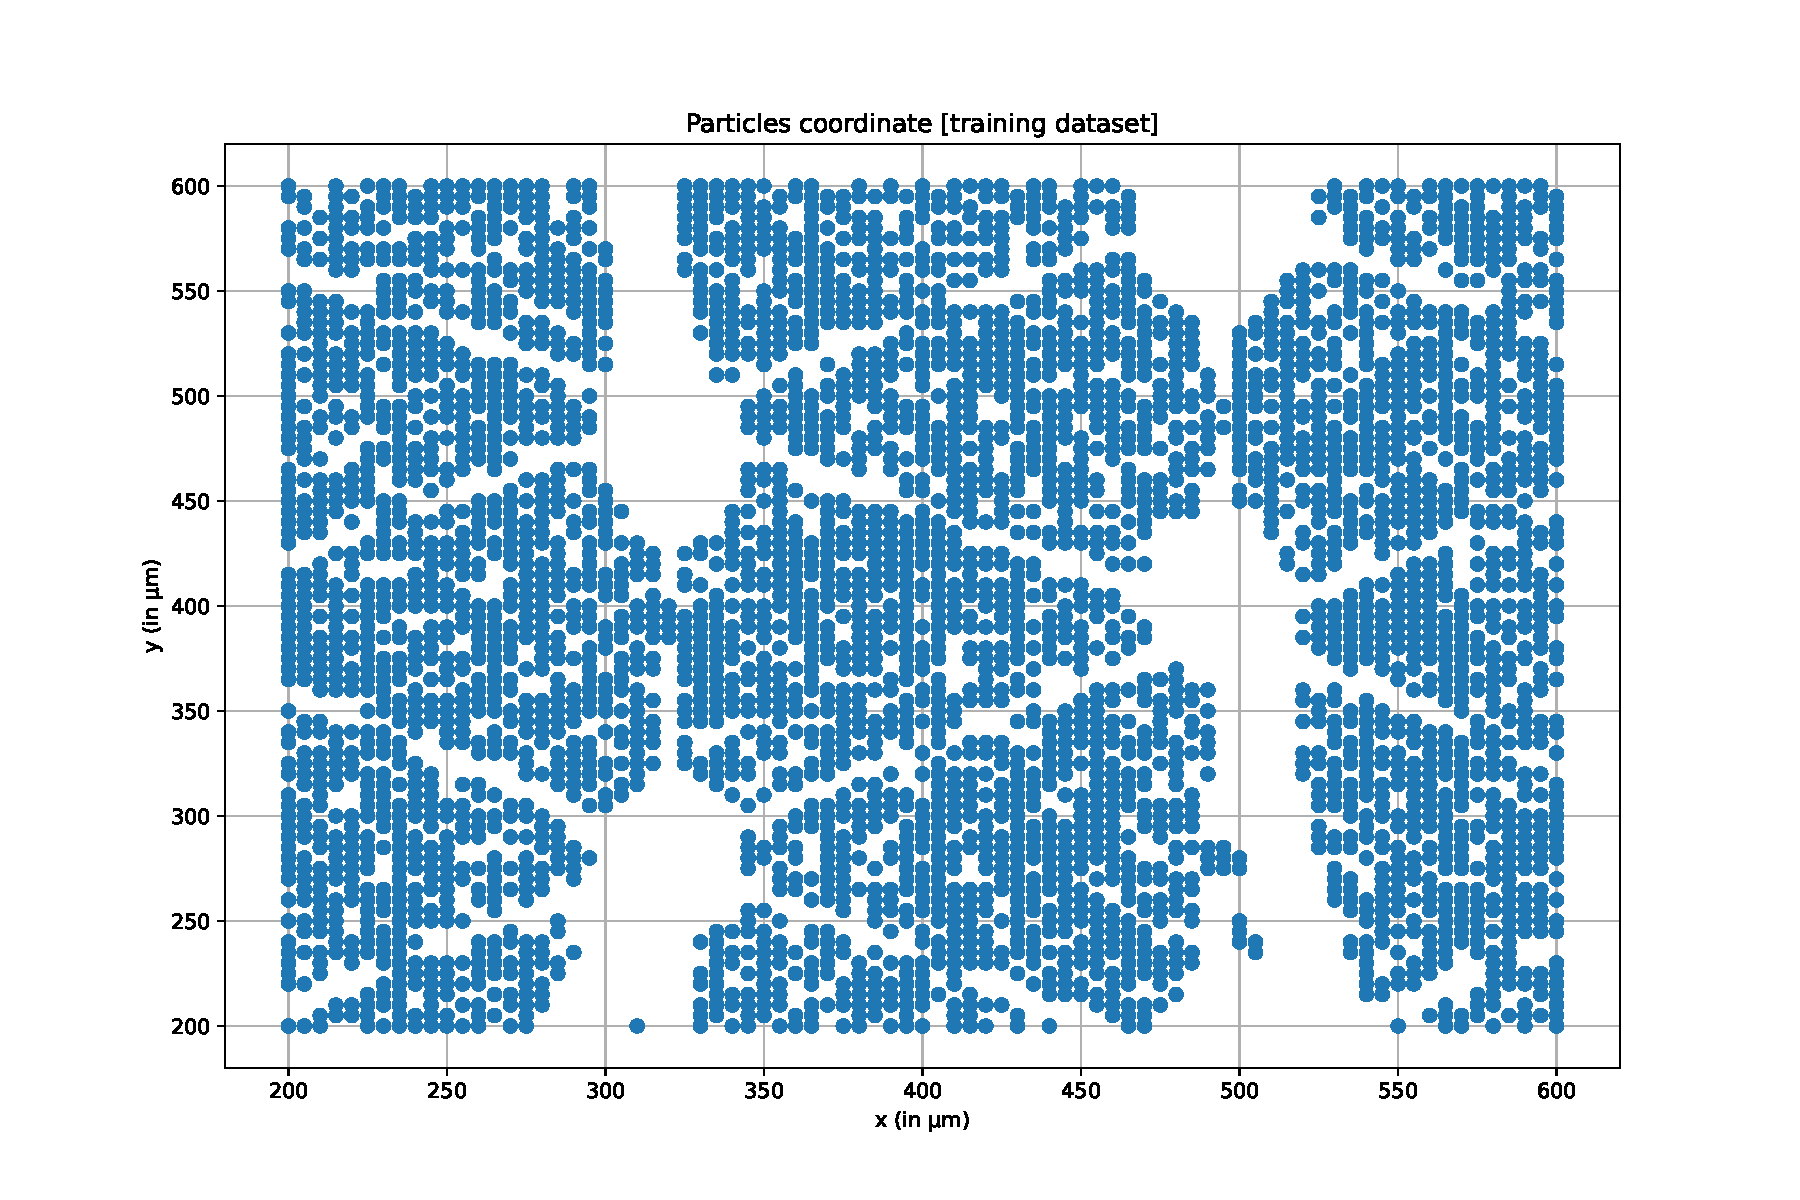
\includegraphics[width=\linewidth]{media/plot_dataset.png}}
\caption{Cartesian plane with the x and y coordinates.}
\label{fig:cartesian_plane}
\end{figure}

The preprocessing phase begins by understanding the utility of all the 5 features extracted 
from the signals exported by the pads.

Feature selection process was employed during the preprocessing phase. After experimenting with 
various feature combinations, it was determined that the model yielded better results when 
trained on a subset of features. \cite{OpenAI_ChatGPT_help_me_on_this}
Features associated with \textit{“tmax”} and \textit{“rms”} were identified as less impactful, 
prompting their removal from the dataset.
This first phase removes 36 columns from the dataset.\\

To mitigate the noise generated from 18 readings across 12 pads, different feature 
selection methods have been implemented and tried with the objective of excluding 
columns that contain features that are noise.

\begin{itemize}
    \item VarianceThreshold: a feature selection method that removes features with low variance, 
    considering them less informative. It was used with \textit{thresholds} equal to 0.35.
    \item SelectKBest: a feature selection approach that selects the top k features based on a scoring function. 
    It was used with \textit{k} equals to 60. This method focuses on retaining the k most informative features.
    \item SelectFwe: (Select Family-Wise Error rate): a feature selection method 
    that controls the family-wise error rate to reduce the likelihood of false discoveries. 
    It was used with the \textit{scoring function} equivalent to \textit{f\_regression}, which assesses the linear 
    relationship between each feature and the target variable. \cite{OpenAI_ChatGPT_help_me_on_this}
\end{itemize}

After experimenting these feature selections methods with different parameters the SelectFwe methods 
was chosen. This feature selection method led to the removal of another 9 columns.\\

After removing all the useless and/or noise features all the remaining columns have been transformed 
in the range 0 to 1, meaning that the minimum and maximum value of a feature is going to be 0 and 1. 
For doing that the MinMaxScaler preprocessing function has been applied to the dataset.


\subsection{Model selection}
In this context of regression analysis, where the objective is to predict continuous numerical values 
a regressor model needs to be used. After performing different tests, the selected model is the 
Random Forest Regressor from scikit-learn's python library.

The RandomForestRegressor is an algorithm belonging to the family of decision tree methods. 
Comprising an ensemble of numerous decision trees, this model excels in capturing complex 
relationships within datasets, making it particularly well-suited for regression tasks. 
Each decision tree in the ensemble independently learns patterns from the data, and the 
final prediction is an average or a weighted sum of predictions 
from individual trees. \cite{OpenAI_ChatGPT_help_me_on_this} 


\subsection{Hyperparameters tuning}
TODO
TABELLA CON I PARAMETRI E I VALORI

\section{Results}
TODO
Here you will present your results (models \& configurations selected, performance achieved)

\section{Discussion}
TODO
Any relevant discussion goes here.

\bibliography{bibliography}
\bibliographystyle{ieeetr}

\end{document}
